\section*{Appendix}

In \cref{chapter5} we omitted some plots in regards to the data generation process which we attach here.

\subsection*{Training anomaly detection on AE-dpMERF data}

\subsubsection*{Using $\epsilon=1$}

\begin{figure}[H]
    \centering
    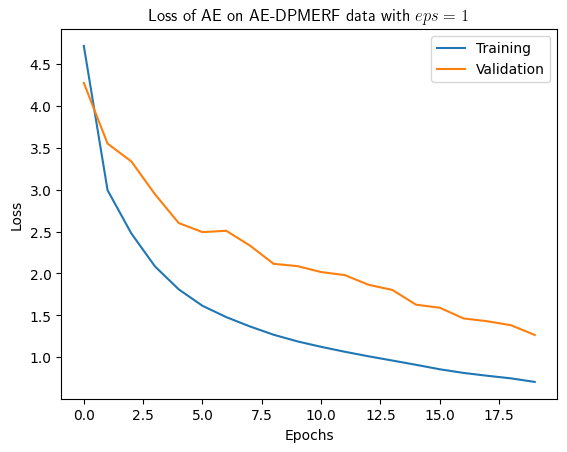
\includegraphics[scale=0.7]{loss_aedpmerf_eps1.png}
    \caption{Loss over epoch for anomaly detection model trained on AE-dpMERF generated data with $\epsilon=1$ together with loss on validation set}
\end{figure}

\begin{figure}[h]
    \begin{minipage}[b]{0.45\textwidth}
        \centering
        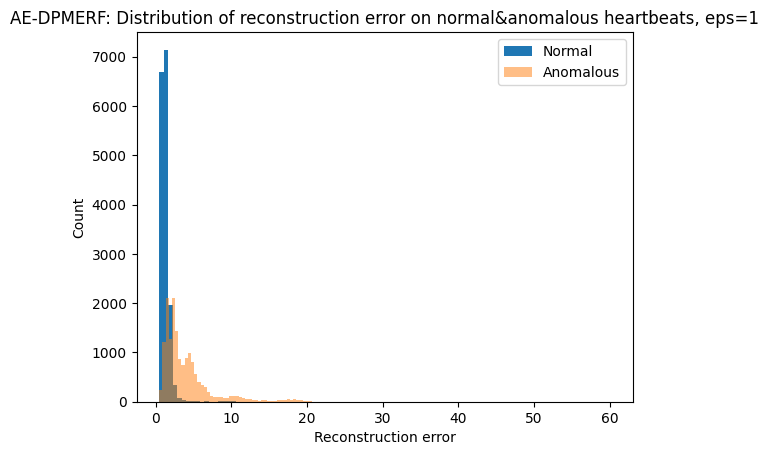
\includegraphics[scale=0.4]{hist_threshold_aedpmerf_eps1.png}
        \caption{Distribution of reconstruction error on validation set with AE-dpMERF with $\epsilon=1$ generated samples}
    
    \end{minipage}
    \begin{minipage}[b]{0.45\textwidth}
        \centering
        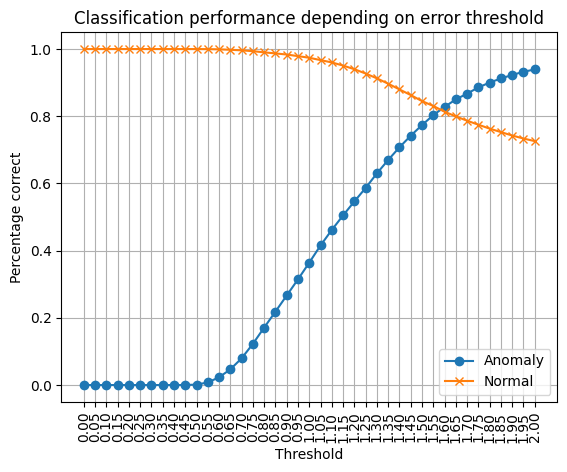
\includegraphics[scale=0.4]{thres_plot_aedpmerf_eps1.png}
        \caption{Percentage of correctly classified regular and anomalous test samples for different threshold values with AE-dpMERF with $\epsilon=1$ generated sampled}
        \label{fig:thres_aegwan}
    \end{minipage}
\end{figure}

\subsubsection*{Using $\epsilon=0.5$}

\begin{figure}[H]
    \centering
    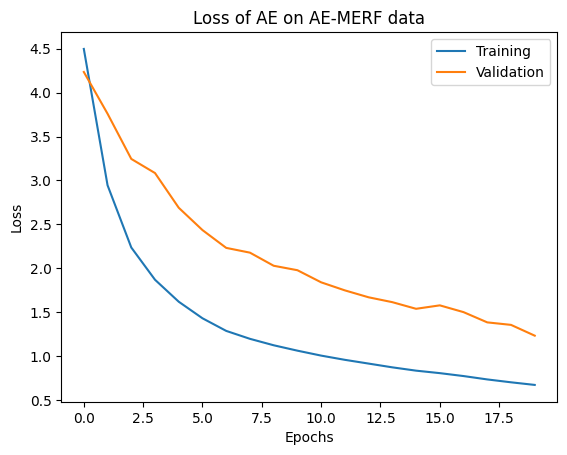
\includegraphics[scale=0.7]{loss_aedpmerf_eps05.png}
    \caption{Loss over epoch for anomaly detection model trained on AE-dpMERF generated data with $\epsilon=0.5$ together with loss on validation set}
\end{figure}

\begin{figure}[h]
    \begin{minipage}[b]{0.45\textwidth}
        \centering
        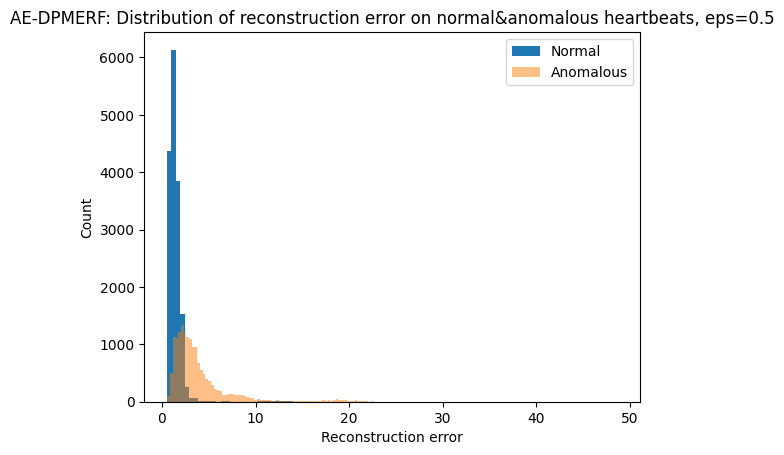
\includegraphics[scale=0.4]{hist_threshold_aedpmerf_eps05.png}
        \caption{Distribution of reconstruction error on validation set with AE-dpMERF with $\epsilon=0.5$ generated samples}
    
    \end{minipage}
    \begin{minipage}[b]{0.45\textwidth}
        \centering
        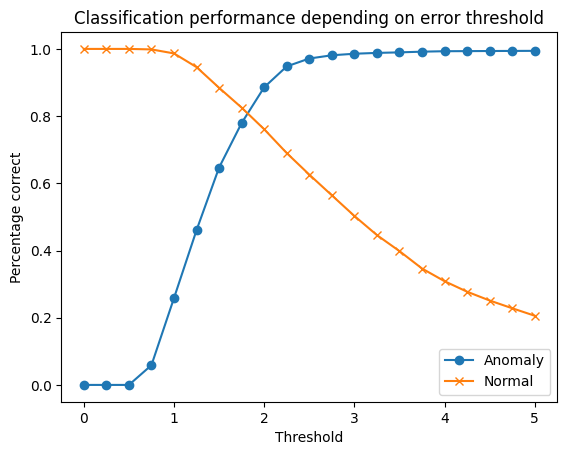
\includegraphics[scale=0.4]{thres_plot_aedpmerf_eps05.png}
        \caption{Percentage of correctly classified regular and anomalous test samples for different threshold values with AE-dpMERF with $\epsilon=0.5$ generated sampled}
        \label{fig:thres_aegwan}
    \end{minipage}
\end{figure}

\subsubsection*{Using $\epsilon=0.1$}

\begin{figure}[H]
    \centering
    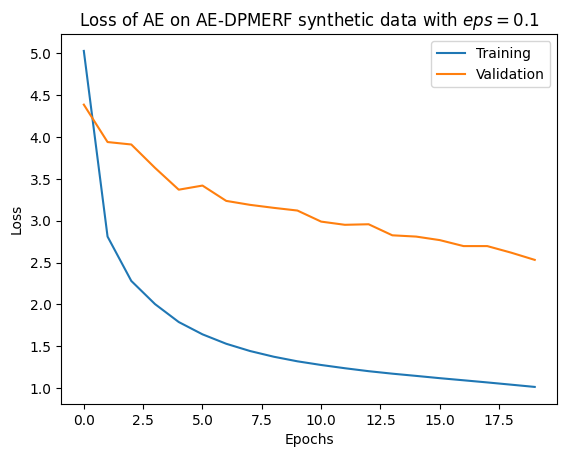
\includegraphics[scale=0.7]{loss_aedpmerf_eps01.png}
    \caption{Loss over epoch for anomaly detection model trained on AE-dpMERF generated data with $\epsilon=0.1$ together with loss on validation set}
\end{figure}

\begin{figure}[h]
    \begin{minipage}[b]{0.45\textwidth}
        \centering
        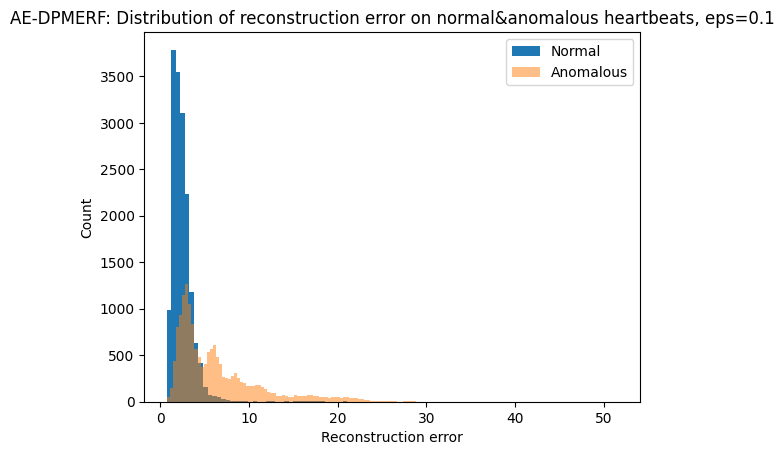
\includegraphics[scale=0.4]{hist_threshold_aedpmerf_eps01.png}
        \caption{Distribution of reconstruction error on validation set with AE-dpMERF with $\epsilon=0.1$ generated samples}
    
    \end{minipage}
    \begin{minipage}[b]{0.45\textwidth}
        \centering
        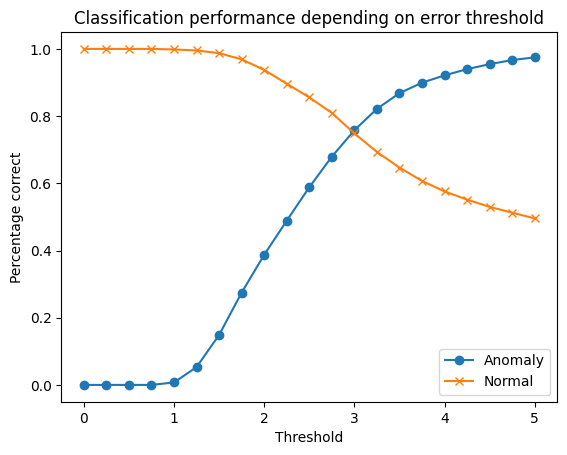
\includegraphics[scale=0.4]{thres_plot_aedpmerf_eps01.png}
        \caption{Percentage of correctly classified regular and anomalous test samples for different threshold values with AE-dpMERF with $\epsilon=0.1$ generated sampled}
        \label{fig:thres_aegwan}
    \end{minipage}
\end{figure}

\subsubsection*{Using $\epsilon=0.01$}

\begin{figure}[H]
    \centering
    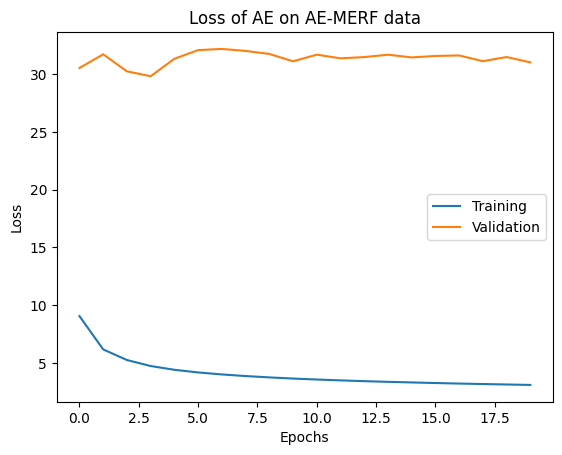
\includegraphics[scale=0.7]{loss_aedpmerf_eps001.png}
    \caption{Loss over epoch for anomaly detection model trained on AE-dpMERF generated data with $\epsilon=0.01$ together with loss on validation set}
\end{figure}

\begin{figure}[H]
    \begin{minipage}[b]{\textwidth}
        \centering
        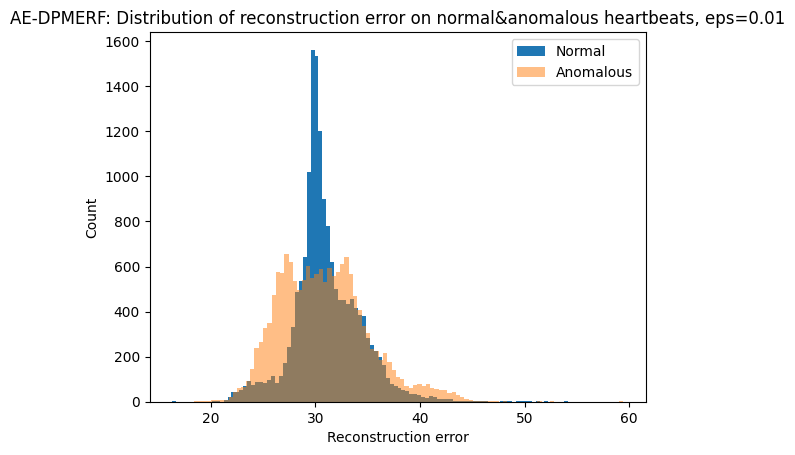
\includegraphics[scale=0.4]{hist_threshold_aedpmerf_eps001.png}
        \caption{Distribution of reconstruction error on validation set with AE-dpMERF with $\epsilon=0.01$ generated samples}
    
    \end{minipage}
    \begin{minipage}[b]{\textwidth}
        \centering
        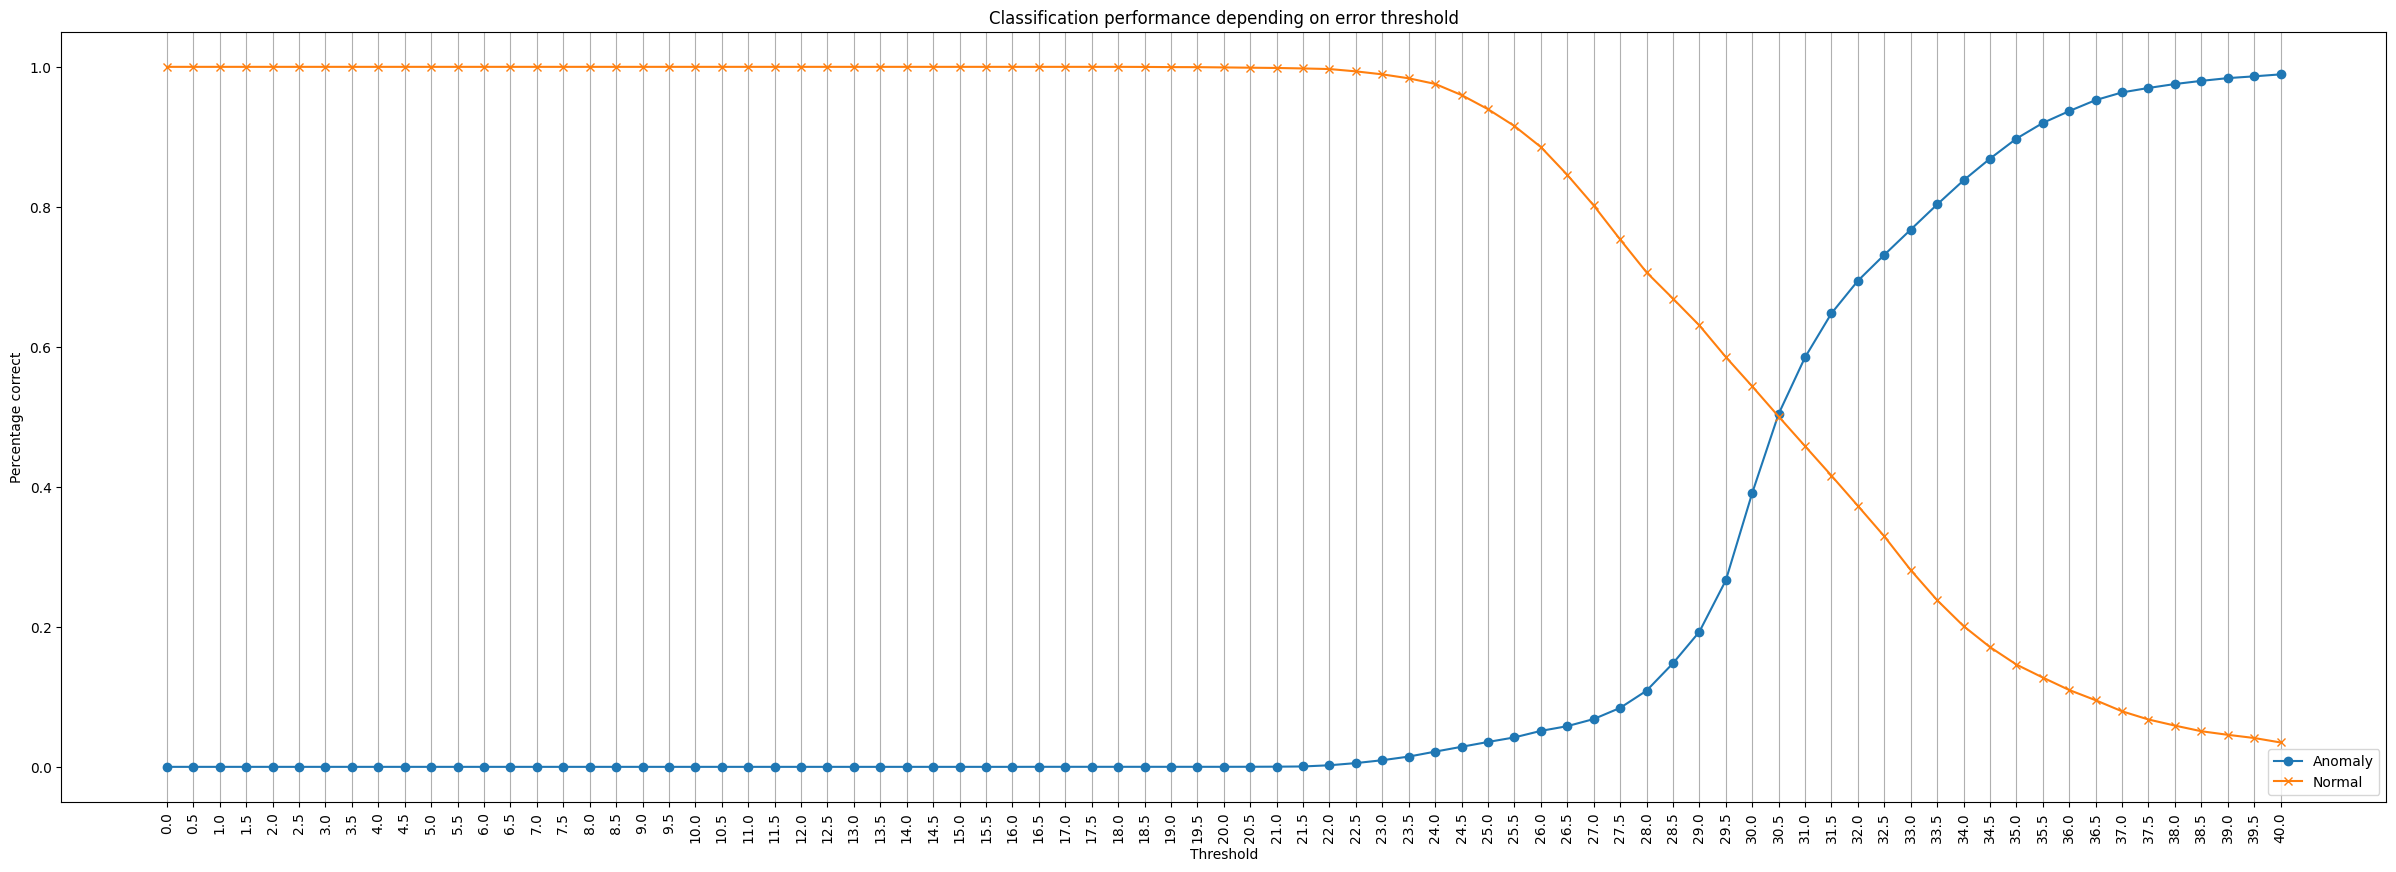
\includegraphics[scale=0.4]{thres_plot_aedpmerf_eps001.png}
        \caption{Percentage of correctly classified regular and anomalous test samples for different threshold values with AE-dpMERF with $\epsilon=0.01$ generated sampled}
        \label{fig:thres_aegwan}
    \end{minipage}
\end{figure}




\subsection*{Training anomaly detection on AE-dpWGAN data}

\subsubsection*{Using $\epsilon=35$}


\begin{figure}[H]
    \begin{minipage}[b]{\textwidth}
        \centering
        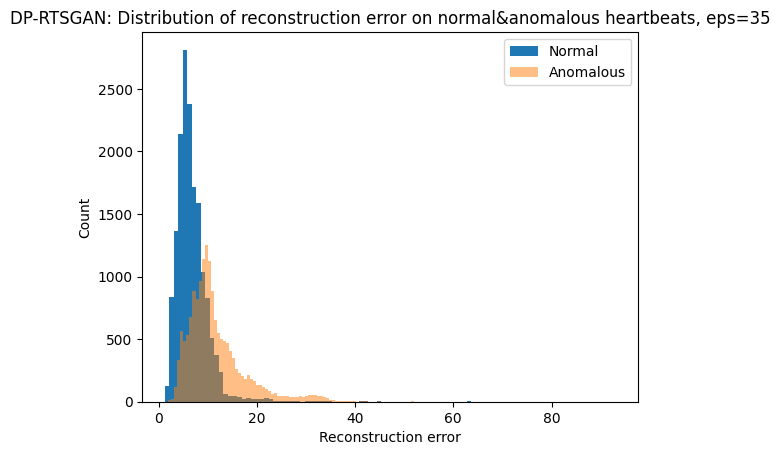
\includegraphics[scale=0.4]{hist_threshold_aedpwan_eps35.png}
        \caption{Distribution of reconstruction error on validation set with AE-dpWGAN with $\epsilon=35$ generated samples}
    
    \end{minipage}
    \begin{minipage}[b]{\textwidth}
        \centering
        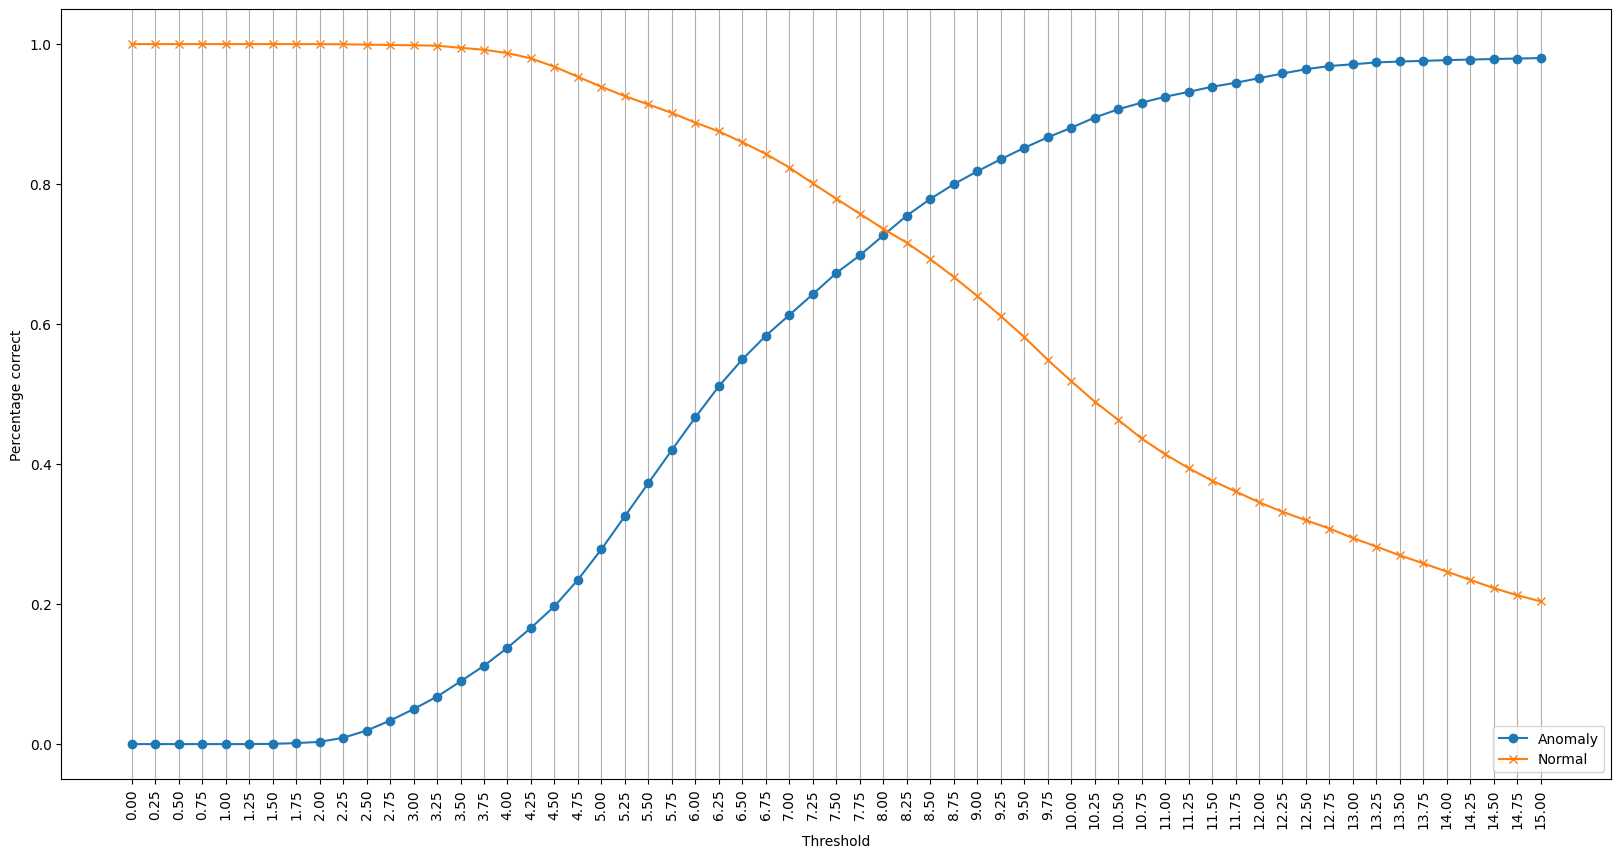
\includegraphics[scale=0.4]{thres_plot_aedpwgan_eps35.png}
        \caption{Percentage of correctly classified regular and anomalous test samples for different threshold values with AE-dpWGAN with $\epsilon=35$ generated sampled}
        \label{fig:thres_aegwan}
    \end{minipage}
\end{figure}

\subsubsection*{Using $\epsilon=25$}

\begin{figure}[H]
    \begin{minipage}[b]{\textwidth}
        \centering
        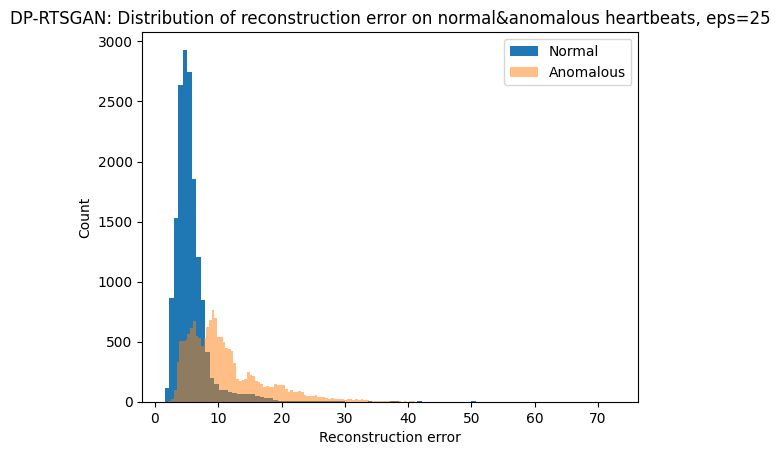
\includegraphics[scale=0.4]{hist_threshold_aedpwgan_eps25.png}
        \caption{Distribution of reconstruction error on validation set with AE-dpWGAN with $\epsilon=25$ generated samples}
    
    \end{minipage}
    \begin{minipage}[b]{\textwidth}
        \centering
        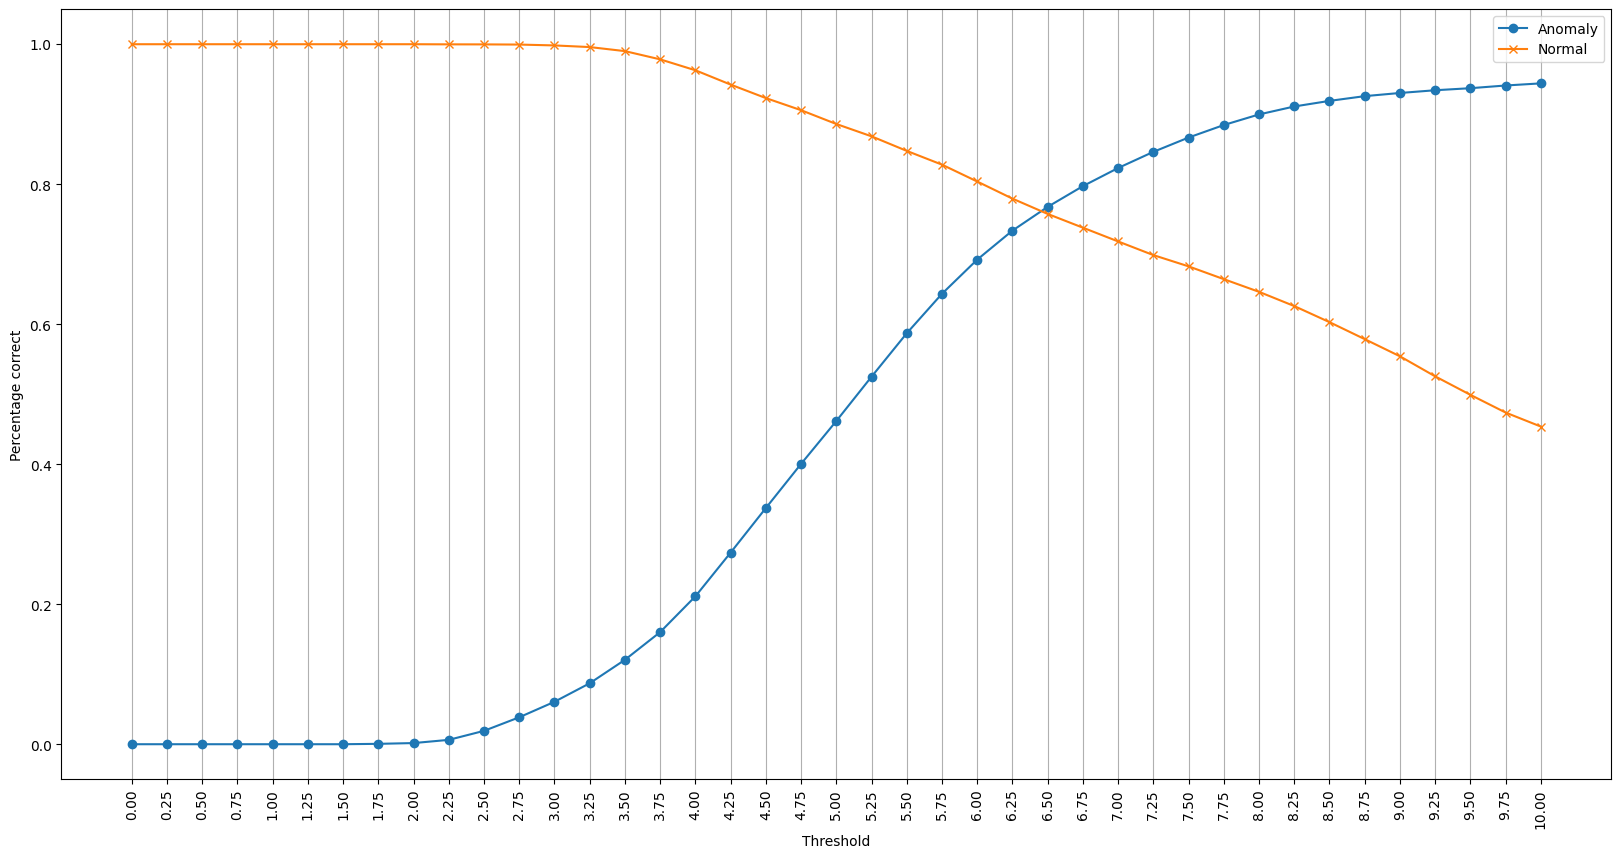
\includegraphics[scale=0.4]{thres_plot_aedpwgan_eps25.png}
        \caption{Percentage of correctly classified regular and anomalous test samples for different threshold values with AE-dpWGAN with $\epsilon=25$ generated sampled}
        \label{fig:thres_aegwan}
    \end{minipage}
\end{figure}

\subsubsection*{Using $\epsilon=5$}


\begin{figure}[H]
        \centering
        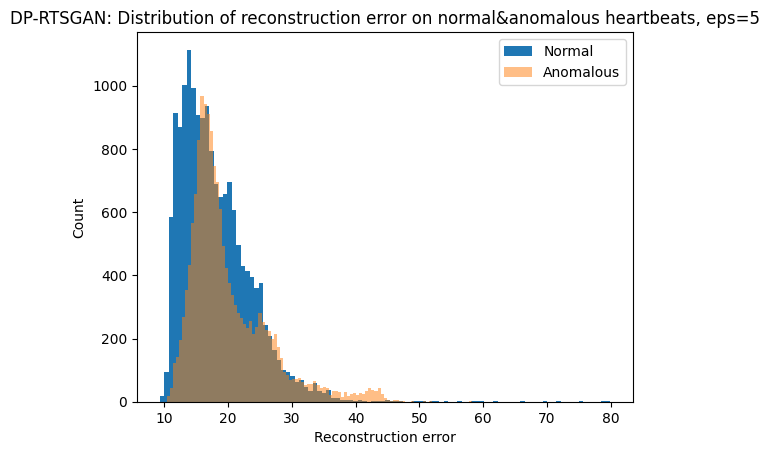
\includegraphics[scale=0.4]{hist_threshold_aedpwgan_eps5.png}
        \caption{Distribution of reconstruction error on validation set with AE-dpWGAN with $\epsilon=5$ generated samples}
\end{figure}

\begin{figure}[H]
        \centering
        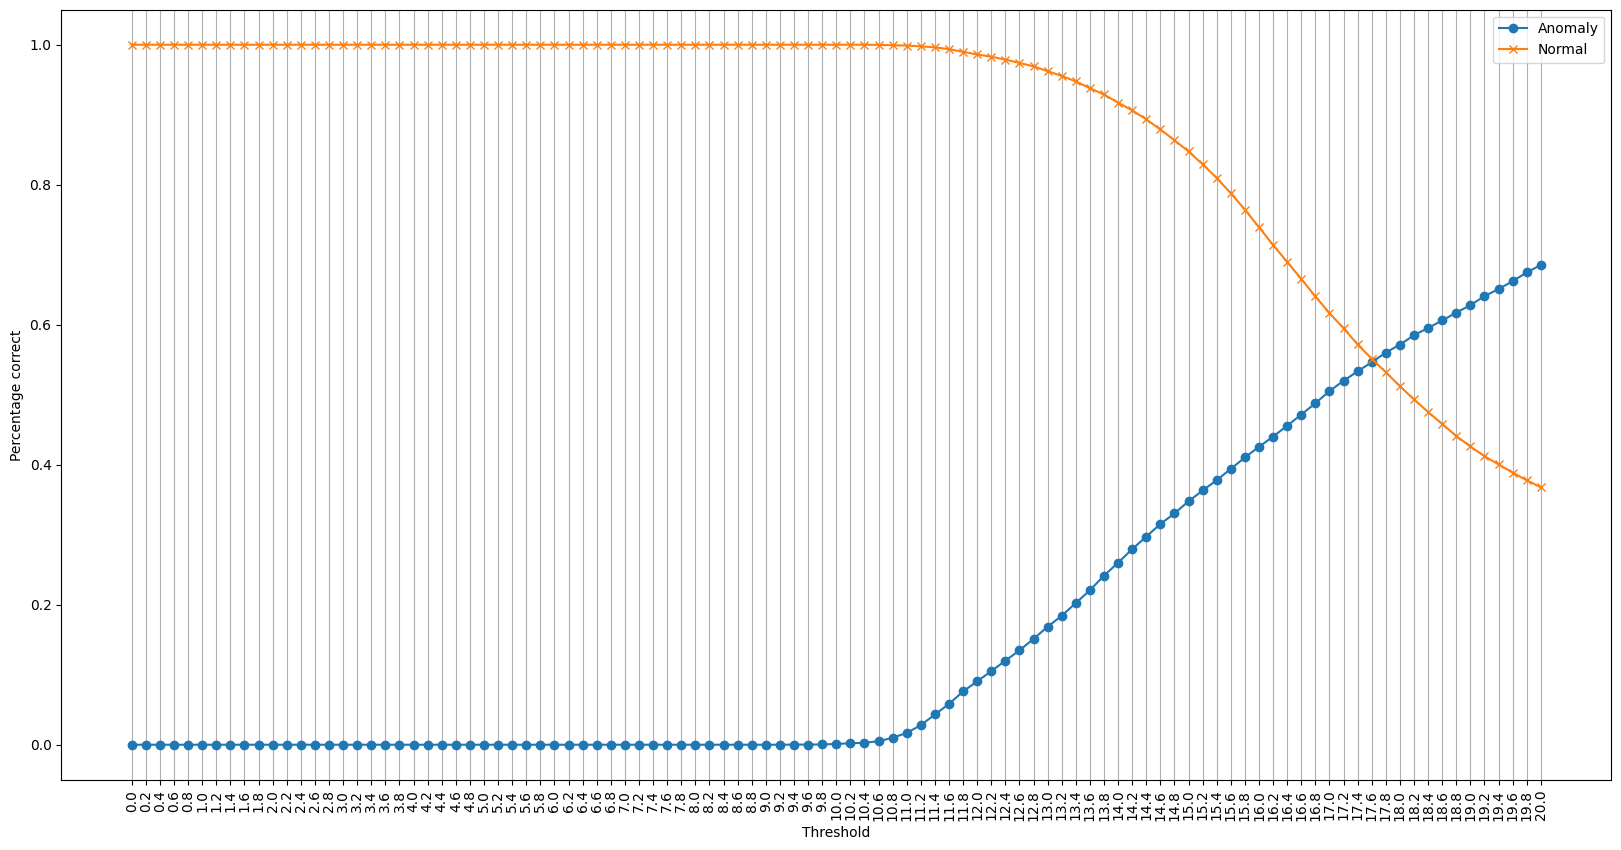
\includegraphics[scale=0.4]{thres_plot_aedpwgan_eps5.png}
        \caption{Percentage of correctly classified regular and anomalous test samples for different threshold values with AE-dpWGAN with $\epsilon=5$ generated sampled}
        \label{fig:thres_aegwan}
\end{figure}